%!TeX program=lualatex
%!TeX spellcheck=en_US
\documentclass[10pt,lualatex,xcolor={table,svgnames},{hyperref={bookmarks=true,linktoc=all}},aspectratio=169]{beamer}
\usetheme{o2report}
\usepackage{amssymb,amsmath}
\usepackage{graphicx}
\graphicspath{{figures/}}
\usepackage{xcolor}
\usepackage{colortbl}
\usepackage{xltxtra}
\usepackage{fontspec}
\usepackage{unicode-math}
\usepackage{appendixnumberbeamer}
\usepackage{wasysym}

\usepackage{csquotes}
\usepackage{pbox}
\usepackage{xhfill}
\usefonttheme{professionalfonts}
\setmainfont{Source Serif Pro}%{Cambria}%
\setsansfont{Source Sans Pro}%{Cambria}%
\defaultfontfeatures{}
\setmonofont{Source Code Pro}%{Cambria}%
\setmathfont{Cambria Math}
%\usepackage{mathastext}
\usepackage{bm,tabu,booktabs,multirow}
\usepackage{ragged2e}
\usepackage{multicol}

\tolerance=100
\setcounter{tocdepth}{3}

\usepackage{xfrac}
\usepackage{xspace,indentfirst}%,paralist}

\setlength{\intextsep}{2pt plus 3pt}% Vertical space above & below [h] floats
\setlength{\textfloatsep}{2pt plus 3pt}% Vertical space below (above) [t] ([b]) floats
\setlength{\abovecaptionskip}{2pt plus 3pt}%
\setlength{\belowcaptionskip}{2pt plus 1pt}%

\usepackage{etoolbox}
\appto\normalsize{%
	\abovedisplayskip=0pt
	\belowdisplayskip=0pt
	\abovedisplayshortskip=0pt
	\belowdisplayshortskip=0pt
}
\appto\small{%
	\abovedisplayskip=0pt
	\belowdisplayskip=0pt
	\abovedisplayshortskip=0pt
	\belowdisplayshortskip=0pt
}

\usepackage[permil]{overpic}

\usetikzlibrary{arrows.meta,graphs,graphdrawing}
\usegdlibrary{layered,trees,force}

%\usetikzlibrary{fit,calc,backgrounds,arrows}
\usepackage{endnotes}
\usepackage{minted}[breaklines=true,bgcolor=LightGray]
\usepackage{lipsum}

\newcommand{\logical}[1]{\textcolor{Green}{#1}}
\newcommand{\programmatic}[1]{\textcolor{-green!40!yellow}{#1}}
\newcommand{\notion}[1]{\textcolor{teal}{#1}}
\newcommand{\operation}[1]{\textcolor{FireBrick}{#1}}

\newcommand{\codelines}[2]{{\mintinline[bgcolor=gray!20,fontsize=#2]{cpp}|#1|}}
\newcommand{\codeline}[1]{{\mintinline[bgcolor=gray!20,fontsize=\footnotesize]{cpp}|#1|}}

\usemintedstyle{rainbow_dash}

\begin{document}
    \author[Anton Alkin]{Anton Alkin}
    \title{\hspace{3em} Introduction into O\textsuperscript{2} \\ \hspace{3em}  Analysis Framework}
    \date[O\textsuperscript{2} Hackaton, 07/12/2021]{HF \& DQ O\textsuperscript{2} Hackatons, 07/12/2021}

    \begin{frame}{}
        \maketitle
    \end{frame}

    \begin{frame}{Outline}
        \begin{columns}
            \begin{column}{0.1\paperwidth}
            \end{column}
            \begin{column}[c]{0.9\paperwidth}
                \begin{itemize}
                    \item {\huge\bfseries Analysis Paradigm Shift}
                    \item {\huge\bfseries Data Model and Data Manipulation}
                    \item {\huge\bfseries Analysis Tasks and Workflows}
                \end{itemize}
                \vspace{1em}
                {\small
                    \begin{description}
                        \item[Official documentation] \href{https://aliceo2group.github.io/analysis-framework/docs/framework/}{https://aliceo2group.github.io/analysis-framework/docs/framework/}
                \end{description}}
            \end{column}
        \end{columns}
    \end{frame}

    \section{New Paradigm}
    \begin{frame}{DPL Analysis Framework}
        \centering%
        \resizebox{\textwidth}{!}{\usetikzlibrary{positioning}
\usetikzlibrary{trees}
\usetikzlibrary{fit}
\begin{tikzpicture}

      \node (transport) [matrix,shape=rectangle,draw,ampersand replacement=\&,fill=blue!20,column sep=5pt]
      {
      		\node[shape=rectangle,draw,fill=cyan!20] (reader) {
      		\texttt{internal-aod-reader}
      		};
      		\&
      		\node[shape=rectangle,draw,fill=magenta!10] (process) {
      		\texttt{o2-analysistutorial-histograms}
      		}; \\
	      \node {};
	      \&
	      \node {\textbf{Transport layer (FairMQ)}}; \\
      };

      \node (task) [matrix,shape=rectangle,draw,fill=blue!20,above=45pt of transport,ampersand replacement=\<,column sep=1pt, row sep=1pt] {
            	      \node {
            	   	\begin{tabular}{c|c|c}
				\rowcolor{green!20}
		      		{} & $Z_{\mathrm{vtx}}$ & $N_{\mathrm{trk}}$ \\
		      		\hline
		      		\rowcolor{green!20}
		      		1 & {} & {} \\
		      		\hline
		      		\rowcolor{green!20}
		      		2 & {} & {} \\
		      		\rowcolor{green!20}
		      		\multicolumn{3}{c}{...}
			\end{tabular}
		      \begin{tabular}{c|c|c}
		      		\rowcolor{red!20}
		      		{} & $p_{\mathrm{T}}$ & $\eta$ \\
		      		\hline
		      		\rowcolor{red!20}
		      		1 & {} & {} \\
		      		\hline
		      		\rowcolor{red!20}
		      		2 & {} & {} \\
		      		\rowcolor{red!20}
		      		\multicolumn{3}{c}{...}
			\end{tabular}
	      };\\
     		\node {\colorbox{magenta!10}{\texttt{void process(\colorbox{green!20}{aod::Collision} const\& c,  \colorbox{red!20}{aod::Tracks} const\& t)}}}; \\
      		\node {\textbf{DPL Analysis Framework}}; \\
      };

      \node [matrix,shape=rectangle,draw,fill=gray!20, left=10pt of transport, column sep=1em] (root) {
	      \node {\colorbox{gray!40}{\textbf{ROOT file(s)}}}; \\
	      \node[shape=rectangle,text width=60pt] (df) {
			DF:
			$-$~\colorbox{green!20}{O2collision}
			$-$~\colorbox{red!20}{O2track}
			$-$~O2muon
			$-$~...
	      }; \\
      };

      \node [matrix,shape=rectangle,draw,fill=gray!20,right=10pt of transport] (output) {
      		\node[fill=gray!40] {\textbf{Output}}; \\
      		\node (histogram) {\includegraphics[width=60pt]{figures/eta.pdf}}; \\
      };

      \node (DPL) [matrix,shape=rectangle,draw,fill=blue!20,above=10pt of transport,,ampersand replacement=\&] {

	      \node {\textbf{Data Processing Layer}}; \\
      };
      \node (shared) [matrix,shape=rectangle,draw,fill=blue!20,below=10pt of transport] {
      		\node [shape=rectangle,draw,fill=green!20] {\texttt{arrow::Table}}; & \node [shape=rectangle,draw,fill=red!20] {\texttt{arrow::Table}}; \\
      		\node {\textbf{Shared memory backend}}; & \node {}; \\
      };

      \draw[-stealth] (root) edge (reader);
      \draw[-stealth] (reader) edge (shared);
      \draw[-stealth] (shared) edge (transport);
      \draw[-stealth] (transport) edge (DPL);
      \draw[-stealth] (DPL) edge (task);
      \draw[-stealth] (process) edge (output);

\end{tikzpicture}}
    \end{frame}

\begin{frame}[shrink=14]{Main differences from Run1/2}
    \vspace{2ex}
    \begin{columns}
        \begin{column}{0.32\textwidth}
            \begin{block}{Data Model}
                \begin{itemize}
                    \item Interconnected Tables instead of containers with object instances
                    \item Reversed access hierarchy: e.g. \logical{Tracks} \emph{refer} to \logical{Collisions}, while previously \logical{Collisions} \emph{contained} \logical{Tracks}
                    \item Optimized for \emph{bulk operations} rather than traditional loops
                    \item Only necessities are stored: processing power is more accessible than disk space
                \end{itemize}
                \smallskip
            \end{block}
        \end{column}
        \begin{column}{0.32\textwidth}
            \begin{block}{Processing Paradigm}
                \begin{itemize}
                    \item \programmatic{Workflow} as a collection of factorized \programmatic{Tasks}, exchanging \programmatic{Tables}, instead of a single Task
                    \item Allows re-using of intermediate data (especially when running on \programmatic{Hyperloop})
                    \item Allows modular analyses constructed from common blocks
                    \item Allows optimization in the background
                \end{itemize}
                \smallskip
            \end{block}
        \end{column}
        \begin{column}{0.32\textwidth}
            \begin{block}{User Interface}
                \begin{itemize}
                    \item Keeps familiar notions of \notion{Analysis Task} and \enquote{objects} -- row accessors to \programmatic{Tables}
                    \item Adjusting for the Data Model differences, allows legacy analysis code to be used with reasonably few modifications
                    \item Provides declarative tools for defining bulk operations without explicit loops and double loops
                    \item \emph{Still in development} -- tell us what your particular analysis needs
                \end{itemize}
                \smallskip
            \end{block}
        \end{column}
    \end{columns}
\end{frame}

\section{Data Model}
\begin{frame}[shrink=11]{Overview}
    \vspace{2ex}
	\begin{columns}
    \begin{column}{0.45\textwidth}
        \begin{block}{How processing is organized}
            \begin{itemize}
                \item \operation{Piping} of data through a set of connected \programmatic{workflows}
                \item \programmatic{Dataframe} as a self-contained unit of processing (following Run3 requirements)
                \item \programmatic{Tasks} process one \programmatic{Dataframe} at once and send out their outputs per-\programmatic{Dataframe}
                \item Data is immutable, \programmatic{Tasks} can only \operation{create} new \programmatic{Tables} or histograms, but not modify existing ones
                \item Data stays in shared memory, single entity accessible to all of the \programmatic{Tasks}
                \item Flattened data structures allow to leverage memory streaming
            \end{itemize}
        \end{block}
    \end{column}
    \begin{column}{0.45\textwidth}
        \begin{block}{How the data is organized}
            \begin{itemize}
                \item \operation{Structure-of-arrays} instead of familiar from Run2 \operation{array-of-structures}
                \item Arrays(referred to as \programmatic{Columns}) are organized in logical \programmatic{Tables}, corresponding to physical concepts of \logical{Collisions}, \logical{Tracks} etc.
                \item \programmatic{Tables} may refer to other \programmatic{Tables} through \programmatic{Index Columns} that contain row numbers
                \item \programmatic{Tables} that correspond row-to-row and have a same number of rows can be \operation{Joined}
                \item \programmatic{Tables} that correspond row-to-row but have a different number of rows can be tied through an \programmatic{Index Table}
            \end{itemize}
        \end{block}
    \end{column}
    \end{columns}
\end{frame}

\begin{frame}[fragile,shrink=5]{Overview (cont.)}
    \vspace{2ex}
	\begin{columns}
    \begin{column}{0.4\textwidth}
        \begin{block}{Some technical details}
            \begin{itemize}
                \item A \programmatic{Table} is defined as a unique C++ type, templated on \programmatic{Columns}, themselves unique C++ types
                \item Underlying contiguous arrays in memory are \emph{immutable} -- no data is removed or copied in common operations such as \operation{Grouping}, \operation{Filtering} or \operation{Partitioning}
                \item \programmatic{Tables} can be read from or written into a ROOT TTree
                \item New \programmatic{Tables} can be defined and created by users
            \end{itemize}
        \end{block}
    \end{column}
    \begin{column}{0.55\textwidth}
        \begin{minted}[bgcolor=gray!30,fontsize=\footnotesize,autogobble]{cpp}
 namespace bc
 {
     DECLARE_SOA_COLUMN(RunNumber, runNumber, int);
     DECLARE_SOA_COLUMN(GlobalBC, globalBC,
     uint64_t);
     DECLARE_SOA_COLUMN(TriggerMask, triggerMask,
     uint64_t);
 } // namespace bc

 DECLARE_SOA_TABLE(BCs, "AOD", "BC",
 o2::soa::Index<>,
 bc::RunNumber, bc::GlobalBC,
 bc::TriggerMask);
 using BC = BCs::iterator;
        \end{minted}
    \end{column}
\end{columns}
\end{frame}

\begin{frame}{Data Model}
     \vspace{-1ex}%
     \centering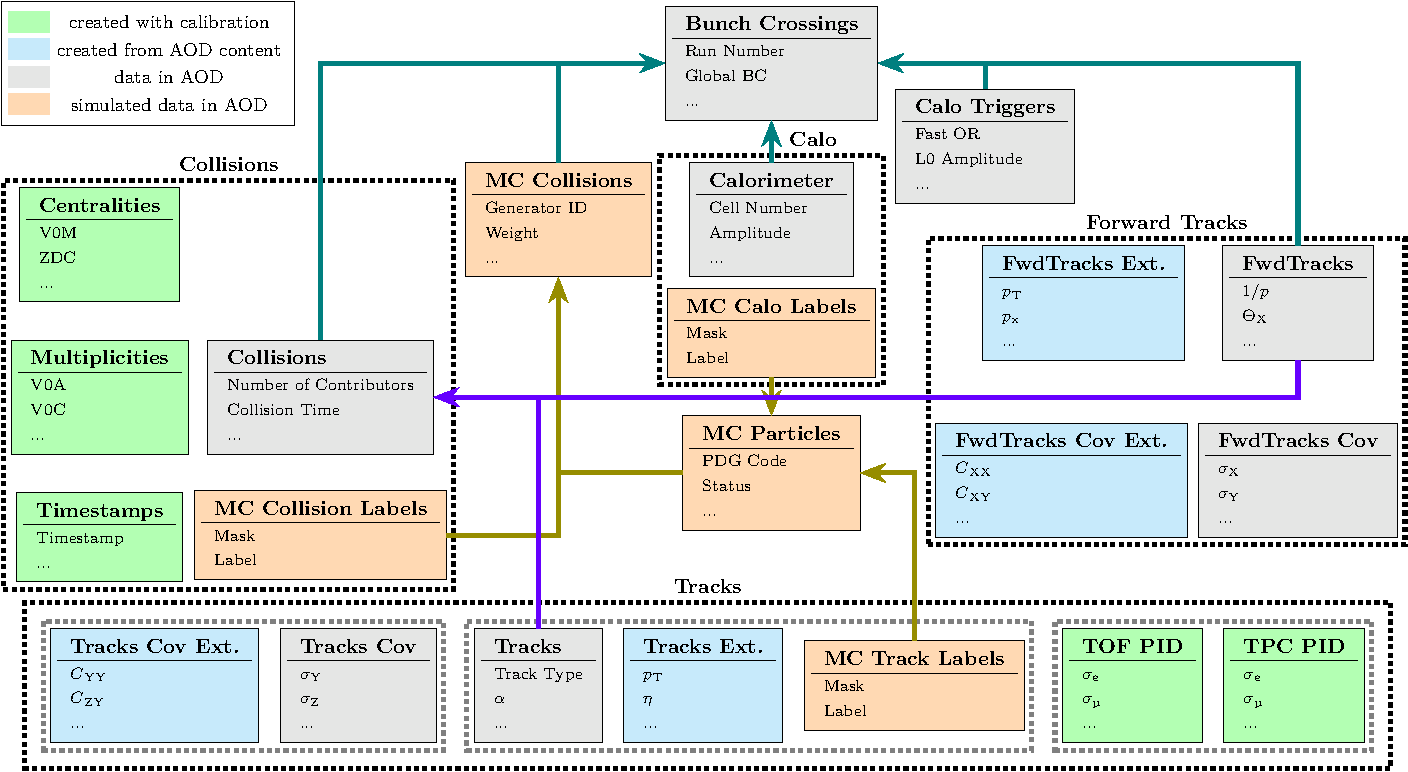
\includegraphics[width=0.9\textwidth]{figures/aod-data-model.pdf}
\end{frame}

\begin{frame}{Data Model (cont.)}%
   \centering \resizebox{!}{0.5\linewidth}{\hspace{-2ex}\usetikzlibrary{positioning}
\newcolumntype{x}{>{\columncolor{green!20}}c}
\newcolumntype{y}{>{\columncolor{red!20}}c}
\newcolumntype{z}{>{\columncolor{blue!20}}c}
\newcolumntype{e}{>{\columncolor{teal!20}}c}
\begin{tikzpicture}
    \matrix[ampersand replacement=\&,column sep=-5pt] {
        \node (tab)  {
       	\renewcommand{\arraystretch}{1.5}
		\begin{tabular}{c|x|x|z|y|e}
			\rowcolor{LightBackground}
			{} & \textbf{X} & \textbf{α}   & $\symbf{f(X,Z,m)}$ & \textbf{Index} & $\symbf{Z=X\sin \alpha}$ \\
			\hline
			1 & {}      & {}     & {}               & \colorbox{cyan!20}{2}    & {} \\
			\hline
			2 & {}     & {}      & {}               & \colorbox{green!20}{3}    & {} \\
			\hline
			{} & \multicolumn{2}{x|}{\large\programmatic{Static}} & {\large\programmatic{Dynamic}} & {\large\programmatic{Index}} & {\large\programmatic{Expression}} \\
			{} & \multicolumn{2}{x|}{\texttt{Arrow::Array}} & {lambda function} & {\texttt{Arrow::Array}} & {\texttt{Arrow::Array}} \\
			{} & \multicolumn{2}{x|}{\texttt{(type, type[N],}} & {not stored in memory} & {} & {created in memory} \\
            {} & \multicolumn{2}{x|}{\texttt{vector<type>)}} & {calculated on demand} & {} & {with Gandiva}
		\end{tabular}
        }; \\
        \node (tab2) {
        	\begin{tabular}{c|c|c}
        	{} & \textbf{A} & \textbf{B} \\
        	\hline
        	1 & {} & {} \\
        	\hline
        	\rowcolor{cyan!20}
        	2 & {} & {} \\
        	\hline
        	\rowcolor{green!20}
        	3 & {} & {}
		\end{tabular}
        };\\
        \& \node {}; \\
};
\end{tikzpicture}}%
\end{frame}

\begin{frame}{Declarations}
%    \vspace{2ex}
\begin{block}{Columns}
    \begin{description}
        \item[Regular] \codeline{DECLARE_SOA_COLUMN(Name,getter,type);}
        \item[Index] \codeline{DECLARE_SOA_INDEX_COLUMN(OriginTable,getter);}
        \item[Dynamic] \codeline{DECLARE_SOA_DYNAMIC_COLUMN(Name,getter,Lambda);}
        \item[Expression] \codeline{DECLARE_SOA_EXPRESSION_COLUMN(Name,getter,type,expression);}
    \end{description}
\end{block}%
\vspace{2ex}
	\begin{block}{Tables}
    \begin{description}
        \item[Regular] \codeline{DECLARE_SOA_TABLE(Name, Origin, Descr,Column1, Column2, ...);}
        \item[Extended] \codeline{DECLARE_SOA_EXTENDED_TABLE(Name,Base,Descr,ExprCol1, ExprCol2, ...);}
        \item[Index] \codeline{DECLARE_SOA_INDEX_TABLE(Name, Key, Descr, IndexCol1, IndexCol2, ..);}
    \end{description}
    \smallskip
\end{block}
\end{frame}

\begin{frame}{Data Manipulation and Filtering}
    \begin{block}{}
        \centering\resizebox{\linewidth}{!}{\usetikzlibrary{positioning}
\newcolumntype{x}{>{\columncolor{green!20}}c}
\newcolumntype{y}{>{\columncolor{red!20}}c}
\usetikzlibrary{arrows}
\begin{tikzpicture}
\node (tab1) {
\begin{tabular}{c|c|c|c|}
{} & X & Y & Z \\
\hline
\rowcolor{green!20} 
1 & {} & {} & {} \\
\hline
\rowcolor{green!20}
2 & {} & {} & {}
\end{tabular}
};
\node (p) [right=1pt of tab1] {$+$};
\node (tab2) [right=1pt of p] {
\begin{tabular}{c|c|c|c|}
{} & A & B & C \\
\hline
\rowcolor{red!20} 
1 & {} & {} & {} \\
\hline
\rowcolor{red!20}
2 & {} & {} & {}
\end{tabular}
};
\node (join) [above=35pt of p] {\LARGE \operation{Join}};
\node (pp1) [below=1pt of p] {};
\node (pp2) [below=25pt of p] {};
\draw [-stealth] (pp1) -- (pp2);
\node (tab3) [below=30pt of p] {
\begin{tabular}{c|x|x|x|y|y|y|}
\rowcolor{LightBackground}
{} & X & Y & Z & A & B & C \\
\hline
1 & {} & {} & {} & {} & {} & {} \\
\hline
2 & {} & {} & {} & {} & {} &{}
\end{tabular}
};

\node (tab4) [right=15pt of tab2] {
\begin{tabular}{c|c|c|c|}
{} & X & Y & Z \\
\hline
\rowcolor{green!20} 
1 & {} & {} & {} \\
\hline
\rowcolor{green!20}
2 & {} & {} & {} \\
\hline
\rowcolor{green!20}
3 & {} & {} & {} \\
\hline
\rowcolor{green!20}
4 & {} & {} & {}
\end{tabular}
};
\node (arr) [right=-5pt of tab4] {};
\node (arr2) [right=10pt of arr] {};
\draw[-stealth] (arr) -- (arr2);
\node (tab5) [right=-2pt of arr2] {
\begin{tabular}{c|c|c|c|}
{} & X & Y & Z \\
\hline
\rowcolor{green!20} 
1 & {} & {} & {} \\
\hline
\rowcolor{red!20}
2 & {} & {} & {} \\
\hline
\rowcolor{red!20}
3 & {} & {} & {} \\
\hline
\rowcolor{green!20}
4 & {} & {} & {}
\end{tabular}
};
\node (filter) [above=35pt of arr] {\LARGE \operation{Filter/Partition}};

\node (tab6) [right=10pt of tab5] {
\begin{tabular}{c|c|c|c|}
{} & X & Y & Z \\
\hline
\rowcolor{green!20} 
1 & {} & {} & {} \\
\hline
\rowcolor{blue!20}
2 & {} & {} & {} \\
\rowcolor{red!20}
3 & {} & {} & {}
\end{tabular}
};
\node (tab7) [right=10pt of tab6] {
\begin{tabular}{c|c|c|c|}
{} & A & B & C \\
\hline
\rowcolor{green!20} 
1 & 1 & {} & {} \\
\rowcolor{green!20} 
2 & 1 & {} & {} \\
\hline
\rowcolor{blue!20}
3 & 2 & {} & {} \\
\rowcolor{blue!20}
4 & 2 & {} & {} \\
\rowcolor{blue!20}
5 & 2 & {} & {} \\
\rowcolor{red!20}
3 & 3 & {} & {}
\end{tabular}
};
\node (gg) [right=5pt of tab6] {};
\node (grouping) [above=35pt of gg] {\LARGE \operation{Grouping}};

\node (tab8) [right=30pt of tab7] {
\begin{tabular}{c|c|c|c|}
{} & X & Y & Z \\
\hline
\rowcolor{green!20} 
1 & {} & {} & {} \\
\hline
\rowcolor{blue!20}
2 & {} & {} & {} \\
\rowcolor{red!20}
3 & {} & {} & {}
\end{tabular}
};
\node (arr3) [below=-5pt of tab8] {};
\node (arr4) [below=10pt of arr3] {};
\draw[-stealth] (arr3) -- (arr4);
\node (tab9) [below=10pt of tab8] {
\begin{tabular}{ccc}
[\colorbox{green!20}{1},\colorbox{blue!20}{2}] & [\colorbox{green!20}{1},\colorbox{red!20}{3}] & [\colorbox{blue!20}{2},\colorbox{red!20}{3}] \\
{[\colorbox{green!20}{1},\colorbox{green!20}{1}]} & [\colorbox{blue!20}{2},\colorbox{blue!20}{2}] & [\colorbox{red!20}{3},\colorbox{red!20}{3}]
\end{tabular}
};

\node (combinations) [above=13pt of tab8] {\LARGE \operation{Combinations}};
\end{tikzpicture}}
    \end{block}
    \begin{block}{}
        \begin{itemize}
            \item {\codeline{soa::Join<aod::Tracks,aod::TracksExtra,aod::TracksCov>}}
            \item {\codeline{soa::Filter<soa::Join<aod::Collisions,aod::Hashes>>}}
            \item {\codeline{void process(aod::Collision const& c, aod::Tracks const& t)}}
            \item {\codeline{for (auto& [t1,t2] : selfCombinations{"fCategory",5,-1,tracks,tracks})}}
        \end{itemize}
    \end{block}
\end{frame}

\begin{frame}{Expressions}
    \begin{block}{}
        {\footnotesize\codeline{Filter f = nabs(aod::track::eta) < etaCut && aod::track::pt > ptCut;}}

        {\footnotesize\codeline{Filter g = (aod::track::flags & someBit != 0);}}

        {\footnotesize\codeline{Partition<Tracks> negative = aod::track::signed1Pt < 0;}}

        {\footnotesize\codeline{DECLARE_SOA_EXPRESSION_COLUMN(Pt, pt, float, nabs(1.f / aod::fwdtrack::signed1Pt));}}
    \end{block}
    \begin{block}{Expressions}
        \begin{itemize}
            \item Almost arbitrary C++ expressions with columns as operands (arithmetic and bitwise operations)
            \item Can be used to define \programmatic{filters} and \programmatic{partitions}, \programmatic{expression columns}
            \item Several math functions can be used (absolute value, trigonometric, square/cubic root, log/exp etc.)
            \item Conditional expressions are available: {\footnotesize\codeline{ifnode(condition, true_exp, false_exp)}}
            \item These are \emph{recipes}, actual computation only happens when needed
        \end{itemize}
    \end{block}
\end{frame}

\begin{frame}{Using tables}
    \begin{block}{Immutable data}
        \begin{itemize}
            \item Underlying data \emph{is never changed}: arrays in shared memory
            \item A \programmatic{Table} is an object, that \emph{views} the data in a certain way
            \item \programmatic{Join} is a \emph{combined view}
            \item \programmatic{Filter/Partition} is a view with a mask
        \end{itemize}
    \end{block}
    \vspace{1.5ex}
    \begin{block}{Iterators}
        \begin{itemize}
            \item An \programmatic{Iterator} (\codeline{Table::iterator}) is an object that views a current \emph{row} of a \programmatic{Table}
            \item It can be used to scroll through the table, access values in the current row, calculate dynamic columns or follow indices from the current row
            \item It is relatively \emph{costly} to construct -- avoid creating iterators in loops -- re-use
            \item Following an index creates an iterator of the target table
        \end{itemize}
    \vspace{0.5ex}
    \end{block}
\end{frame}

\begin{frame}[shrink=3]{Creating tables}
    \vspace{1em}
    \begin{block}{Declaration}
        \begin{itemize}
            \item Tables are defined by their C++ type and attached static metadata
            \item All tables have to be declared, user tables can be added just as the ones in the core data model
            \item User-defined extended and index tables use \codeline{*_USER()} version of the macros and their creation needs to be explicitly requested
        \end{itemize}
    \end{block}
    \begin{block}{Derived, Extended and Index tables}
        \begin{description}
            \item [\codeline{Produces<DerivedTable> cursor;}] Derived tables are directly filled, row by row, by calling the cursor, created by \codeline{Produces<>} template. Table is only created after the filling task finishes.
            \item [\codeline{Spawns<ExtendedTable> handle;}] User-defined extended tables need to be requested by adding \codeline{Spawns<>} template to the task. The table is created before the task is run and is accessible through the \codeline{handle} variable.
            \item [\codeline{Builds<IndexTable> handle;}] User-defined Index tables need to be requested by adding \codeline{Builds<>} template to the task. The table is created before the task is run and is accessible through the \codeline{handle} variable.
        \end{description}
    \end{block}
\end{frame}

\section{Analysis Task}
\begin{frame}[fragile]{Analysis Task}
    \centering
    \begin{tabular}{p{0.1\textwidth}p{0.8\textwidth}}
        {\rotatebox[origin=r]{90}{\centering \programmatic{Boilerplate} \ \ \ \ \ }} & {\scriptsize
            \begin{minted}[linenos,breaklines]{c++}
#include "Framework/runDataProcessing.h"
#include "Framework/AnalysisTask.h"

using namespace o2;
using namespace o2::framework;
                \end{minted}
            } \\
            {\rotatebox[origin=r]{90}{\centering \programmatic{Task} \ \ \ \ \ }} & {\scriptsize
                \begin{minted}[linenos,breaklines,autogobble,firstnumber=6]{c++}
struct MyTask {
    ...
};
            \end{minted}
        } \\
    {\rotatebox[origin=r]{90}{\centering \programmatic{Boilerplate} \ \ \ \ }} & {\scriptsize
        \begin{minted}[linenos,breaklines,autogobble,firstnumber=10]{c++}
WorkflowSpec defineDataProcessing(ConfigContext const& cfgc)
{
    return WorkflowSpec{
        adaptAnalysisTask<MyTask>(cfgc)
    };
}
        \end{minted}
    }
    \end{tabular}
\end{frame}

\begin{frame}[fragile]{Analysis Task}
    \centering
    \begin{tabular}{p{0.1\textwidth}p{0.8\textwidth}}
        {\rotatebox[origin=r]{90}{\centering \programmatic{Declarative} \ \ \ \ \ \ \ \ \ \ \ \ }} & {\scriptsize
            \begin{minted}[linenos,breaklines,autogobble]{c++}
struct MyTask {
    Produces<MyTable> mt;            //
    Spawns<MyExtension> me;          // Creation of new tables
    Builds<MyIndex> mi;              //
    HistogramRegistry registry{"registry",
        {{"h","h",{HistType::kTH1F, {{10, -1, 1}}}}}
    };
    Filter f = track::pt > 0.5;
    Configurable<float> etaCut{"etaCut", 1.0f, "eta cut"};
    Filter e = nabs(track::eta) < etaCut;
    Partition<Tracks> negativeSide = track::eta < 0;
                \end{minted}
            } \\
            {\rotatebox[origin=r]{90}{\centering \programmatic{Imperative} \ \ \ \ \ \ \ }} & {\scriptsize
                \begin{minted}[linenos,breaklines,autogobble,firstnumber=13]{c++}
    void process(Collision const& col, soa::Filtered<Tracks> const& tracks){
        ...
        mt(col1, col2, col3);
        ...}
    void anotherProcess(McCollision const& mccol, McParticles const& particles){};
    PROCESS_SWITCH(MyAnalysisTask,anotherProcess,"Process MC", false);
}
            \end{minted}
        }
    \end{tabular}
\end{frame}

\begin{frame}{Declarative features}
    \begin{block}{Configurables}
        \begin{itemize}
            \item A variable that can be set externally: single, 1d array, 2d array, labeled 2d array
            \item Can be set via command line, JSON configuration and via Hyperloop interface
        \end{itemize}

    \end{block}
    \begin{block}{Process switches}
        \begin{itemize}
            \item Boolean configurable with a special purpose: enabling/disabling process functions
            \item Can only be set via JSON or on Hyperloop
        \end{itemize}

    \end{block}
    \begin{block}{Filters, Partitions}
        \begin{itemize}
            \item Selections on incoming data, that should be calculated upfront, before the task's code is entered
            \item \programmatic{Filters} are automatically tied to all compatible inputs (for all process functions) and logically multiplied if needed
            \item \programmatic{Partitions} are independent selections, that can be used via declared variable
        \end{itemize}

    \end{block}
\end{frame}

\begin{frame}[fragile]{Task ouputs}
    \begin{block}{Histogram Registry}
        \begin{itemize}
            \item Efficient container for histogram objects (\texttt{TH1} descendants and \texttt{THnSparse})
            \item Allows to declare histograms without creating them directly
        \end{itemize}
        \begin{minted}[fontsize=\small,breaklines]{cpp}
HistogramRegistry registry{
    "registry",
    {
        {"eta", "; #eta", {HistType::kTH1F, {{102, -2.01, 2.01}}}},
        {"phi", "; #varphi", {HistType::kTH1F, {{100, 0., 2. * M_PI}}}}
    }
};
        \end{minted}
    \end{block}
    \begin{block}{Output Object}
        \begin{itemize}
            \item Wrapper for generic \texttt{TObject} descendants
        \end{itemize}
\begin{minted}[fontsize=\small]{cpp}
OutputObj<CorrelationContainer> same{"sameEvent"};
OutputObj<CorrelationContainer> mixed{"mixedEvent"};
\end{minted}
    \end{block}
\end{frame}
\section{Summary}

\begin{frame}{Summary}
\begin{itemize}
    \item At the current stage Analysis Framework contains wide set of basic tools to define arbitrary analysis
    \item A number of declarative features is already implemented, leveraging advantages of the flattened data model and bulk processing
    \item \enquote{Traditional} object-like interface is provided to iterate over tables
    \item Work is ongoing to simplify syntax and extend functionality for all of the framework components (which requires more workforce)
    \item \textcolor{DarkGoldenrod}{We need user feedback -- to learn what needs to be improved, or what features are needed the most, and, of course, what problems are there}
\end{itemize}
\end{frame}
\end{document}
